
%%% Local Variables:
%%% mode: latex
%%% TeX-master: t
%%% End:
\section{数据分析的``武器库''}

\begin{frame}{\textcolor{white}{空白}}

  \begin{columns}
    \begin{column}{.5\textwidth}
      \begin{figure}
        \centering 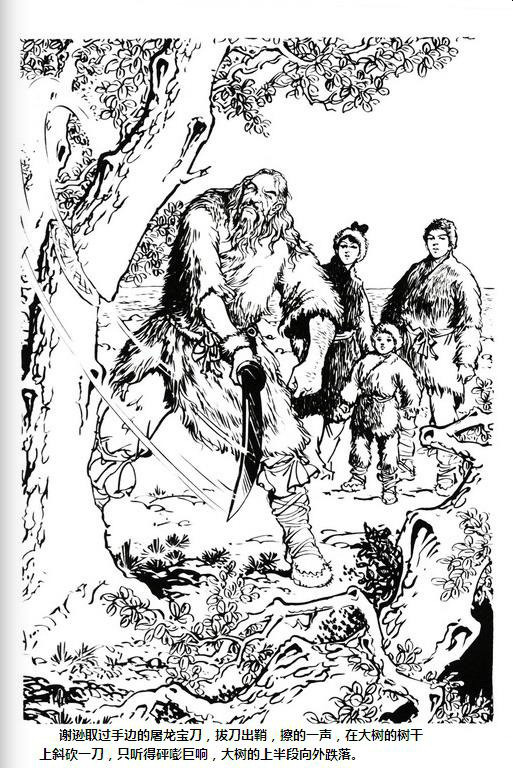
\includegraphics[width=0.95\columnwidth]{chp03_屠龙宝刀.jpg}
      \end{figure}
    \end{column}

    \begin{column}{.5\textwidth}
      \begin{ornamentblock}
        \centering
        {工欲善其事,必先利其器
          \rightline{\textemdash 《论语·卫灵公》}}
      \end{ornamentblock}
    \end{column}
  \end{columns}

\end{frame}

\begin{frame}{数据分析的``七种武器''}
\begin{enumerate}\large
\item 数据采集
\item 数据处理
\item 数据建模
\item 数据库
\item 业务分析
\item 分析算法
\item 可视化
\end{enumerate}
\end{frame}

\subsection{数据采集}
\begin{frame}[t]{\subsecname}
\begin{itemize}
\item<2-> 利用服务器端提供的API接口调取数据
\item<3-> 编写爬虫程序,从网页上抓取数据
\end{itemize}

\begin{overlayarea}{\textwidth}{\textheight}
  \begin{onlyenv}<2>
\begin{figure}
  \centering
  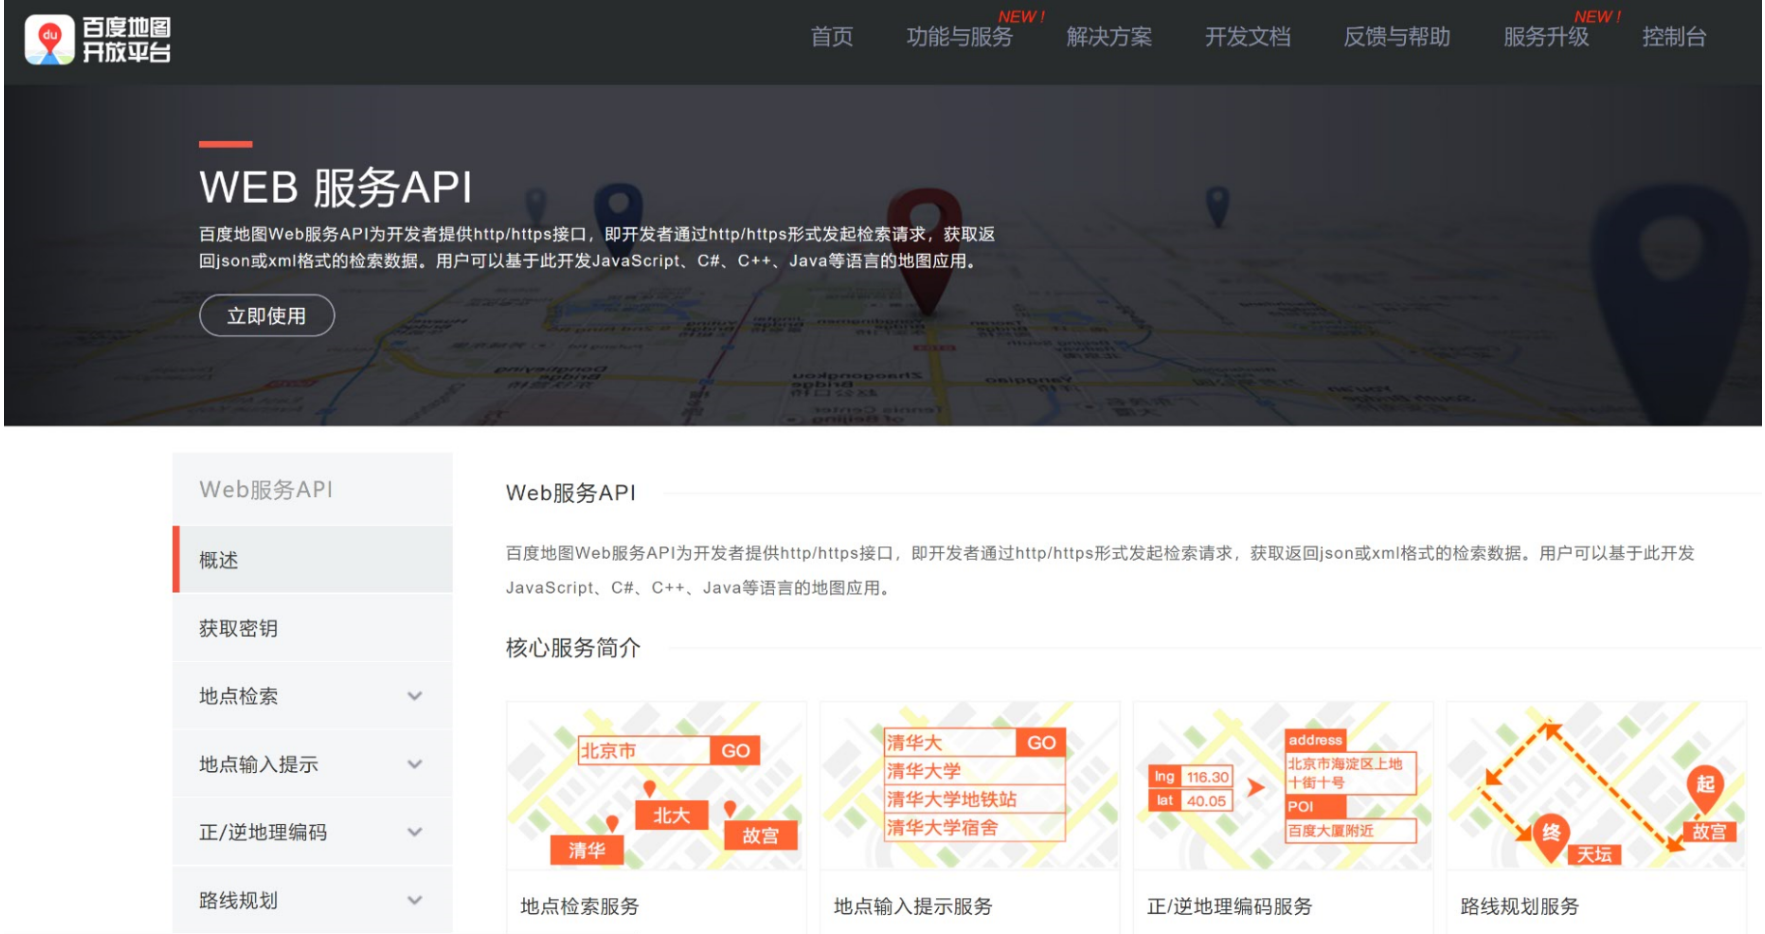
\includegraphics[width=\textwidth]{chp03_百度地图API.png}
  \caption{百度地图提供API接口供用户调取其相应的数据}
\end{figure}
  \end{onlyenv}

\vspace{-15pt}
  \begin{onlyenv}<3>
\begin{figure}
  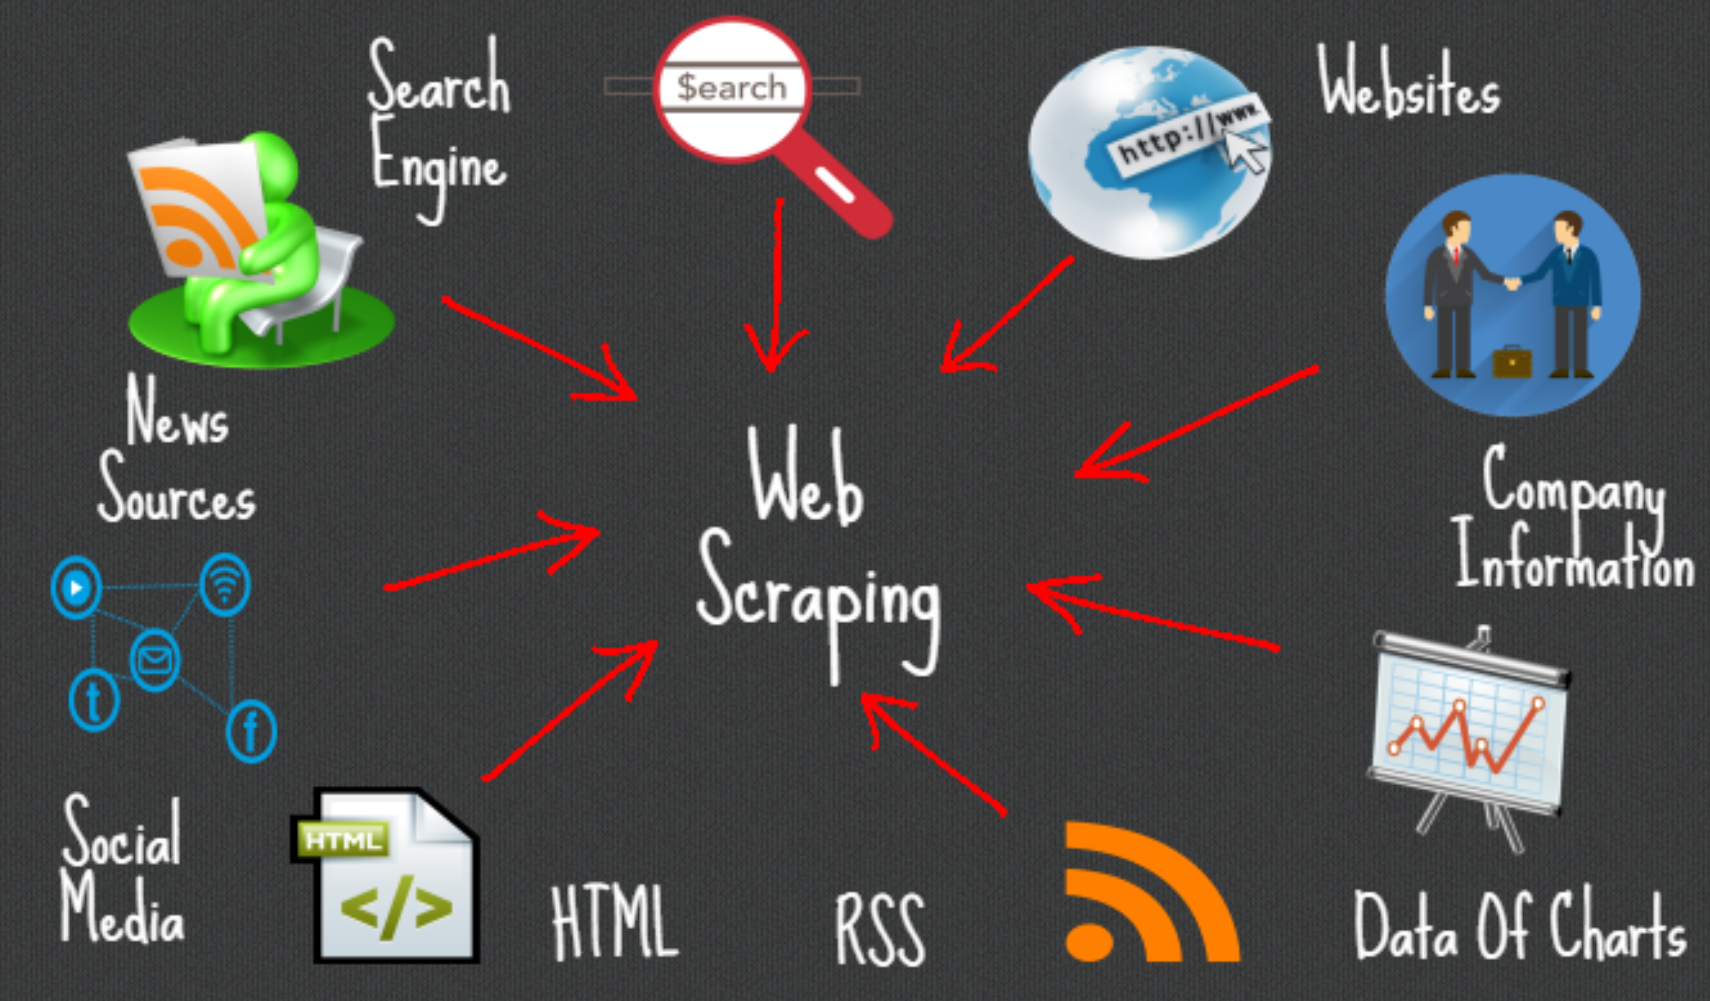
\includegraphics[width=\textwidth]{chp03_网络爬虫.png}
  \caption{利用爬虫程序,可以从广袤的互联网资源中自动化采集数据}
\end{figure}
  \end{onlyenv}
\end{overlayarea}

\end{frame}

\subsection{数据预处理}
\begin{frame}[t]{\subsecname}
\begin{itemize}
\item<1-> 现实中的原始数据都是不完整、不一致的脏数据,需要编写程序对数据进行清洗、集成、变换和归约等自动化处理
\item<2-> 示例:GPS数据与道路的地图匹配
\end{itemize}
\end{frame}

\subsection{数据建模}
\begin{frame}[t]{}
\begin{itemize}
\item<1-> \emphText{根据业务需求对数据进行抽象},形成计算机能够理解的逻辑关系和物理结构
\item<2-> 示例:车辆行驶轨迹模型 
\end{itemize}
\end{frame}

\subsection{数据库}
\begin{frame}[t]{}
\begin{itemize}
\item<1-> 通过高效的组织和存储,便于对数据进行新增、删除、修改和查询等操作
\item<2-> 根据数据量级、数据格式选择最适合的数据库技术
\end{itemize}
\end{frame}

\subsection{业务分析}


\subsection{分析算法}
\begin{frame}[t]{}
\begin{itemize}
\item<1-> 算法不是简单的数据统计,而是要能够挖掘数据背后的规律和关系
\item<2-> 交通规划中最常用的分析算法是\emphText{空间分析算法}
\end{itemize}

\end{frame}


\subsection{可视化}
\begin{frame}[t]{\subsecname}
\begin{itemize}
\item<1-> 计算机可视化技术与艺术的结合体
\item<2-> 用既直观又简洁的图形来展现分析成果
\end{itemize}

\end{frame}

